\chapter{Evaluation}
\label{sec:evaluation}

% Zu jeder Arbeit in unserem Bereich gehört eine Leistungsbewertung. Aus
% diesem Kapitel sollte hervorgehen, welche Methoden angewandt worden,
% die Leistungsfähigkeit zu bewerten und welche Ergebnisse dabei erzielt
% wurden. Wichtig ist es, dem Leser nicht nur ein paar Zahlen
% hinzustellen, sondern auch eine Diskussion der Ergebnisse
% vorzunehmen. Es wird empfohlen zunächst die eigenen Erwartungen
% bezüglich der Ergebnisse zu erläutern und anschließend eventuell
% festgestellte Abweichungen zu erklären.

% Checked
This chapter will evaluate the implementation of the developed
system with respect to performance, design and flexibility.  The
evaluation has emphasis on determining the overhead of CAL and GVON
configured with the MPI adapter in comparison to plain MPI.

It is expected that the overhead is negligible. Therefore, it will
make no difference exchanging MPI with a GVON implementation. So that,
communication processes will be as fast as the underlying adapter
implementation.

The evaluation is divided in several benchmarks and every benchmark
provides several experiments. Synthetic benchmarks will evaluate
solely single communication methods. Instead, real world benchmarks
will compare the implemented simulations in comparison to equivalent
MPI implementations. Thereby will experiments vary in amount of peers,
number of messages to send, number of elements to send, and usage of
network.

The benchmark system was the HPC system of the Helmholz
Zentrum Dresden Rossendorf (HZDR)\cite{ref:hzdr_cluster}.
%% and the
%% system of the Zentrum für Informationsdienste und Hochleistungsrechnen
%% (ZIH).
A part of the HZDR system is the hypnos linux cluster (Ubuntu 12.04.4
LTS) consisting of two head nodes and more than 150 compute nodes.
The so-called laser nodes combine 4 AMD Interlagos Opterons by 4
sockets on a single mainboard resulting in 64 CPUs per node.  The
Interlagos Opterons 6276 are two Valencia chips on a single die,
whereby 2 core share a 64 KB L1 Cache and a 2 MB L2 Cache. Laser nodes
are interconnected by an Infiniband network. These nodes are utilized
in for all synthetic and real simulation benchmarks.

%% In turn, are
%% kepler nodes equipped with 2 Quad-Core Xeon CPUs from Intel clocked by
%% 2,4 GHz. These nodes are used if only a pair of peers is necessary for
%% a benchmark.

%% The ZIH system provides a cluster called taurus. The nodes are
%% equipped each with two Intel Xeon(R) CPU : sandy E5-2690 (8 cores),
%% gpu E5-2450 (cores), west X5660 (6 cores).

The nodes provide their software environment by the module system.
The developed system is compiled with MPI in version 1.8.0 and
g++ 4.8.2.  

% Hier bisschen mehr

%%%%%%%%%%%%%%%%%%%%%%%%%%%%%%%%%%%%%%%%%%%%%%%%%%%%%%%%%%%%%%%%%%%%%%%%%%%%%%%%
%                                                                              %
% SYNTHETIC POINT TO POINT BENCHMARK                                           %
%                                                                              %
%%%%%%%%%%%%%%%%%%%%%%%%%%%%%%%%%%%%%%%%%%%%%%%%%%%%%%%%%%%%%%%%%%%%%%%%%%%%%%%%
% Checked
\section{Synthetic Point to Point Benchmark}
This synthetic benchmark compares the run-time of fundamental
point-to-point communication operations of MPI with CAL and GVON
operations. It is determined the run-time overhead of the CAL and GVON
in respect to the plain usage of MPI. Since this benchmark does not
represent a real world application, it does only contain communication
operations of the particular communication library. The source code of
the experiments is free from any application dependent logic.

Two peers are exchanging data. Whereby one peer is the sender and the
other is the receiver. The run-time is measured for sending and
receiving of $n$ messages with $m$ elements.  A single element is set
fixed to a 64 Bit integer.  An experiment will be called send/recv
operation in the further benchmark description. Every send/recv
operation is executed 100 times and averaged afterwards to reduce
variations in the run-time. An experiment configuration has the
following parameters:

\begin{itemize}
  \item Number of consecutive send/recv operations $n$
  \item Number of elements per send/recv operation $m$
  \item Communicating with or without network
\end{itemize}

\noindent The following experiments, vary a single parameter while the
others stay fixed. This should evaluate the impact of this parameter
with respect to the MPI implementation.

\subsection*{Increase the Number of Consecutive Send/Recv Operations}
% Checked
This experiment increases the number of consecutive send/recv
operations $n$ from 1 to $10^3$ by a step size of 10. The number of
elements per send/recv operation is restricted to a single
element. The run-time for these consecutive send/recv operations is
measured and averaged to obtain the run-time for a single operation.
The experiment is limited on a single node. Therefore, no network
latency is included in the results.  Figure \ref{fig:nsend_kepler}
shows the averaged run-time on a single kepler node and the according
run-time ration in respect to MPI.

\begin{figure}[H]
  \begin{minipage}[t]{0.5\textwidth} 
    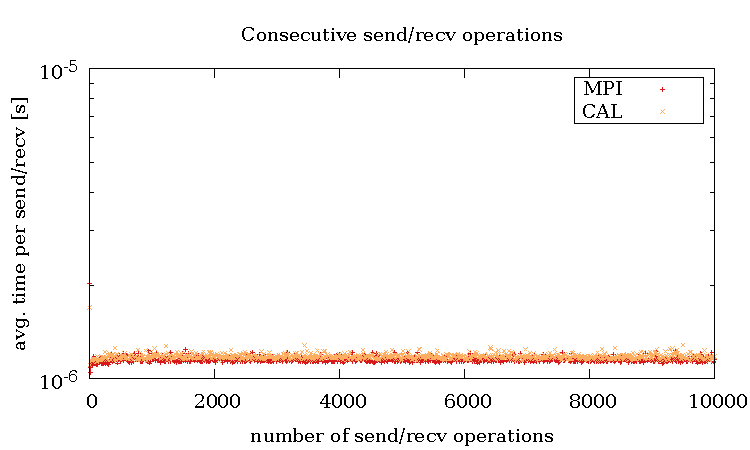
\includegraphics[width=\textwidth]{plots/50_nsend_cal_laser}
    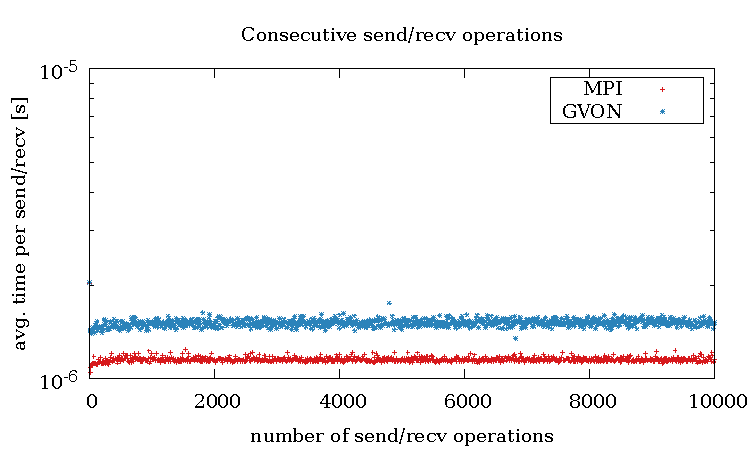
\includegraphics[width=\textwidth]{plots/50_nsend_gvon_laser}
    \end{minipage}%
  \begin{minipage}[t]{0.5\textwidth}
    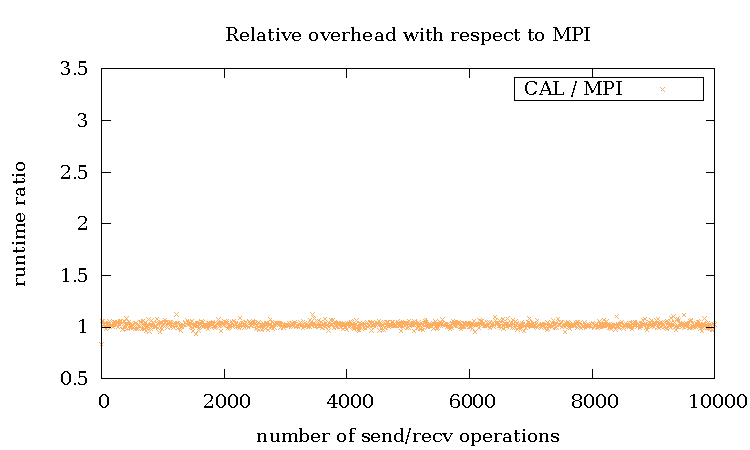
\includegraphics[width=\textwidth]{plots/50_nsend_overhead_cal}
    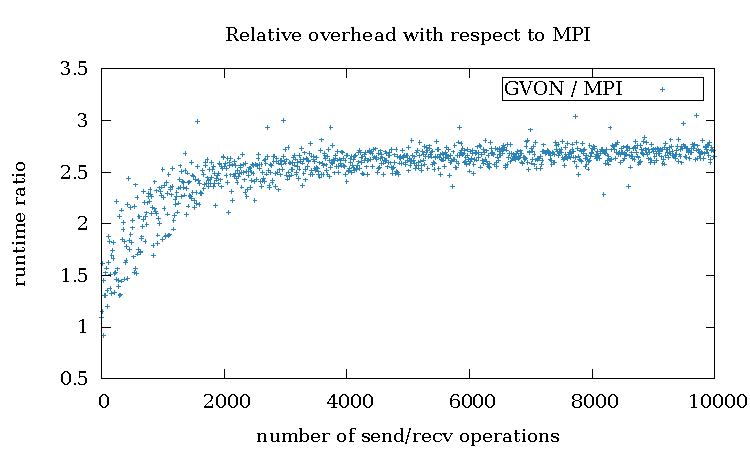
\includegraphics[width=\textwidth]{plots/50_nsend_overhead_gvon}
  \end{minipage}%
  \caption{Average run-time of a single send/recv operation and the
    according overhead of CAL and GVON compared to MPI. The number of
    consecutive operations is increased from 1 to $10^3$ by a step
    size of 10. }
  \label{fig:nsend_kepler}
\end{figure}

\noindent The relative overhead of the CAL and GVON stabilize with
increasing number of send/recv operations.  Through virtual address
and context translations, the CAL adds a constant average overhead of
around 2\% per send/recv operation with respect to MPI. The GVON adds
a constant average overhead of around 30\% per send/recv operation.
Since the communication topology of the GVON is modeled by a graph,
containing two nodes connected by a directed edge, the constantly look
up of this graph adds a constant overhead to each send/recv operation.
Instead, the CAL and MPI are sending and receiving without the need of
a look up from fixed peer addresses .  However, because the graph is
not changing during the experiment, it is sufficient to perform the
graph look up only once. Experiments performed with only one graph
look up will be named GVON OGL. The GVON OGL should reduce overhead to
the similar level of the CAL. Figure \ref{fig:nsend_one_lookup_kepler}
shows the results of the experiment that only performs one look up per
$n$ send/recv operation.

\begin{figure}[H]
  \begin{minipage}[t]{0.5\textwidth} 
    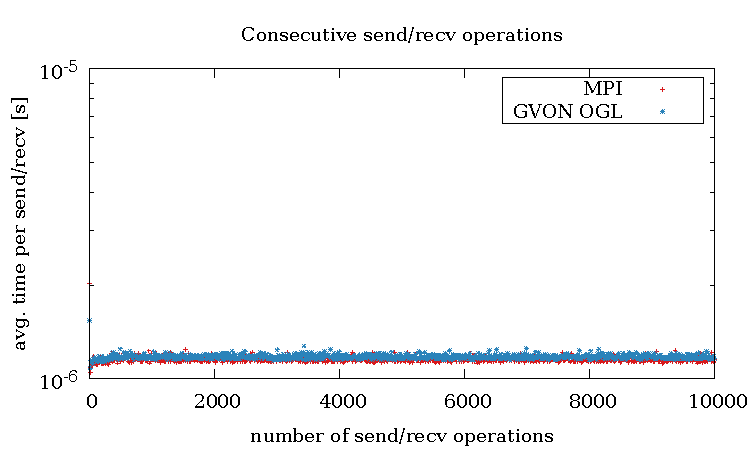
\includegraphics[width=\textwidth]{plots/50_nsend_one_lookup_laser}
  \end{minipage}%
  \begin{minipage}[t]{0.5\textwidth}
    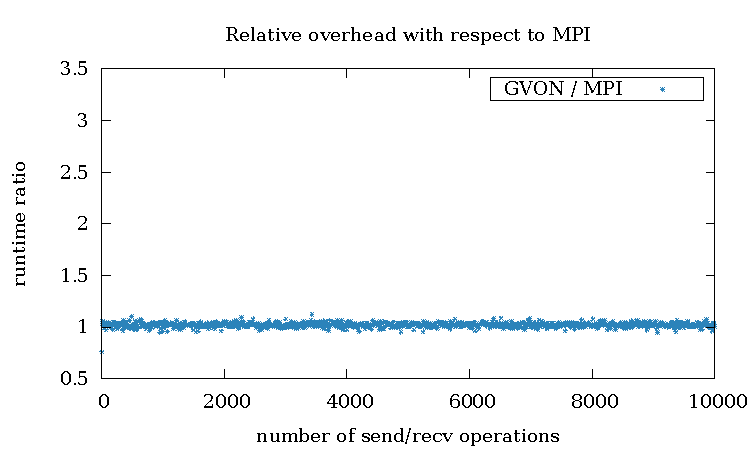
\includegraphics[width=\textwidth]{plots/50_nsend_one_lookup_overhead_gvon_laser}
  \end{minipage}%
  \caption{The amount of graph look ups is reduced to one look up for
    $n$ send/recv operations.  This reduces the GVON overhead to
    a similar level of the CAL.}
  \label{fig:nsend_one_lookup_kepler}
\end{figure}

\noindent Changing the experiment, reduced the GVON overhead to the
same level of the CAL (around 2\%). Nevertheless, the vertex and
graph need to be translated to virtual address and context, so that, a
small overhead in respect to the CAL is still present. It shows that
the graph implementation need to be optimized with regard to look up
of incoming and outgoing edges in the future development.

% Checked
\subsection*{Increase the Number of Elements per Send/Recv Operation}
This experiment increases the number of elements per send/recv
operation from 1 to $10^3$ by a step size of 10. A single experiment
obtains the average run-time over 1000 operations.  The experiment is
limited to execution on a single node. Thus, no network latency is
included in the results. Figure \ref{fig:nsize_kepler} shows the
averaged run-time of a send/recv operation for a single element and
the run-time ration in respect to MPI on a single kepler node.

\todo{Explain run-time jump}
\begin{figure}[H]
  \begin{minipage}[t]{0.5\textwidth}
    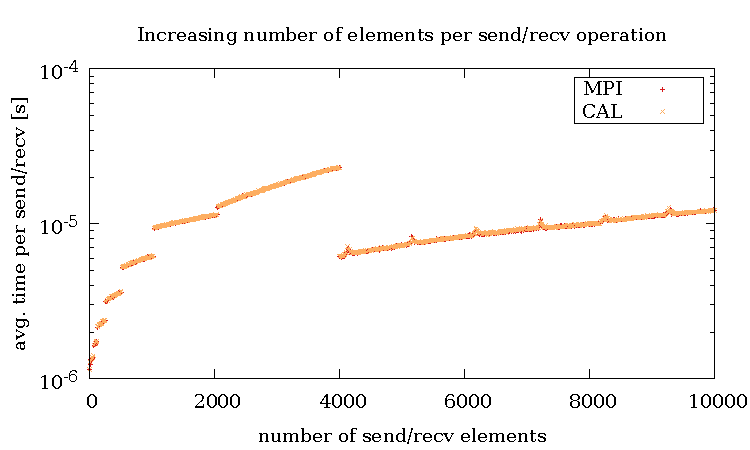
\includegraphics[width=\textwidth]{plots/50_nsize_cal_laser}
    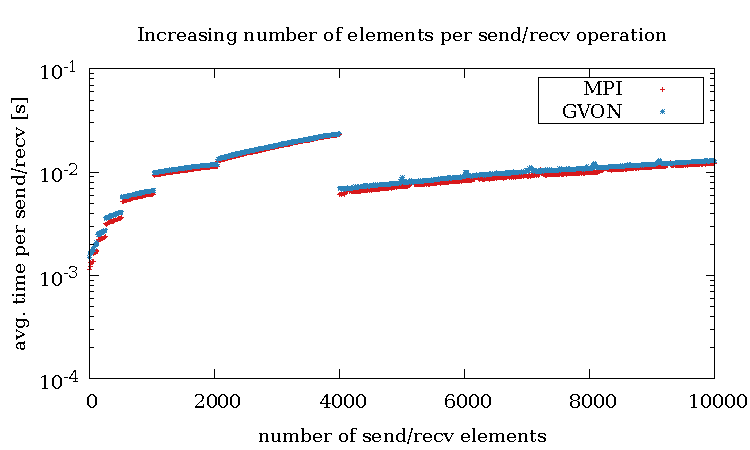
\includegraphics[width=\textwidth]{plots/50_nsize_gvon_laser}
    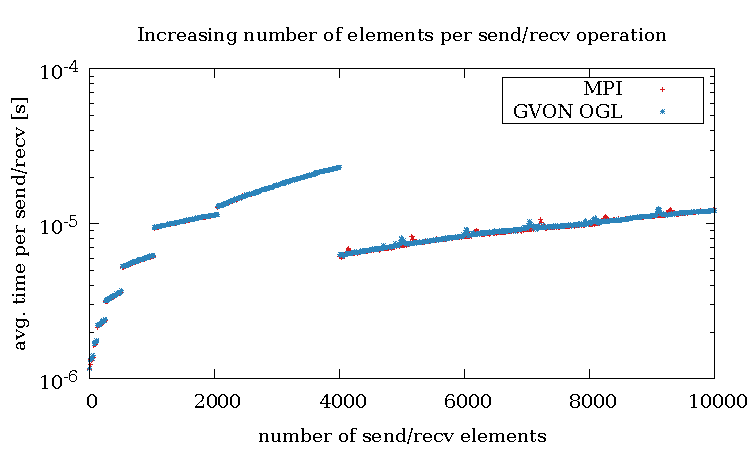
\includegraphics[width=\textwidth]{plots/50_nsize_one_lookup_gvon_laser}
  \end{minipage}%
  \begin{minipage}[t]{0.5\textwidth}
    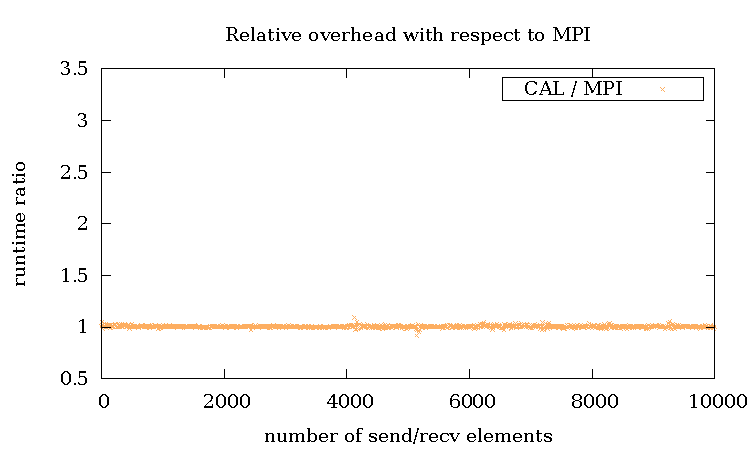
\includegraphics[width=\textwidth]{plots/50_nsize_overhead_cal_laser}
    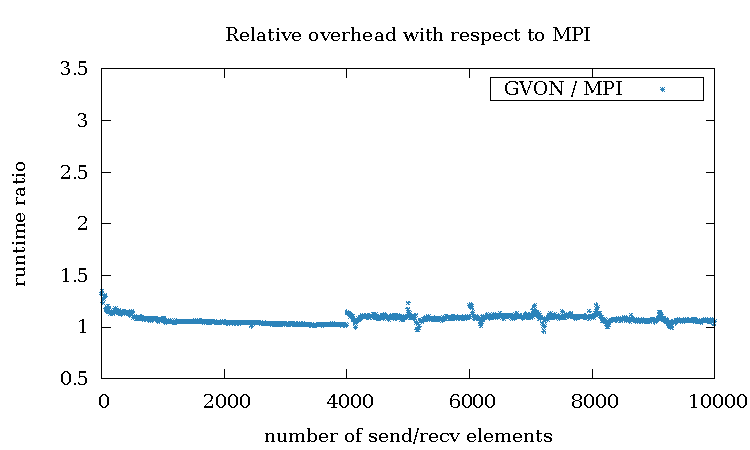
\includegraphics[width=\textwidth]{plots/50_nsize_overhead_gvon_laser}
    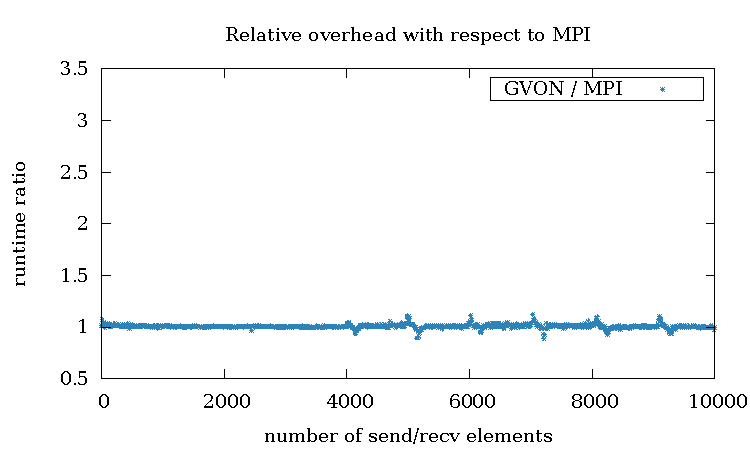
\includegraphics[width=\textwidth]{plots/50_nsize_one_lookup_overhead_gvon_laser}
  \end{minipage}%
  \caption{Increasing the number of elements per send/recv operations,
    reduces the relative overhead in respect to MPI.}
  \label{fig:nsize_kepler}
\end{figure}

\noindent With increasing number of elements per send/recv operations,
the run-time of CAL and GVON converges with the run-time of MPI. The
average CAL overhead is negligible (less then 1\%) and the average
GVON overhead is reduced to around 7\% per send/recv operation. The
last pair of Figures shows, that changing the GVON experiment to a one
graph look up variant, drops the GVON run-time overhead to a
negligible level.

% Checked
\subsection*{Including Network}
The synthetic benchmarks above were performed only locally on a single node.
Therefore, the run-time results were not influenced by network latency.
The experiments setup is changed to a configuration with two
nodes, whereby the peers are not located on the same node. It is
expected, that the relative overhead of CAL and GVON decreases even
more in contrast to the previous experiments, while the overall
run-time will increase.  A setup of two laser nodes, each hosting one
peer, was selected.  Figure \ref{fig:nsend_network} shows the average
run-time of GVON and CAL in respect to MPI for a single send/recv
operation including network latency.

\todo{Repeat experiment with GVON OGL version and decide which experiment to illustrate}
\begin{figure}[H]
  \begin{minipage}[t]{0.5\textwidth}
    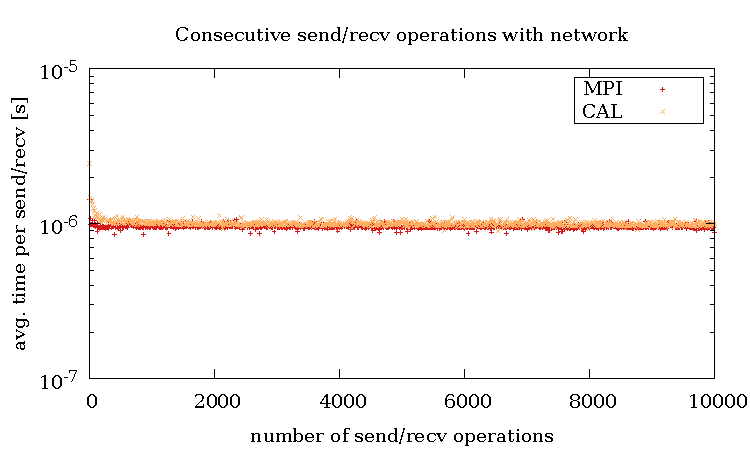
\includegraphics[width=\textwidth]{plots/50_nsend_network_cal_laser}
    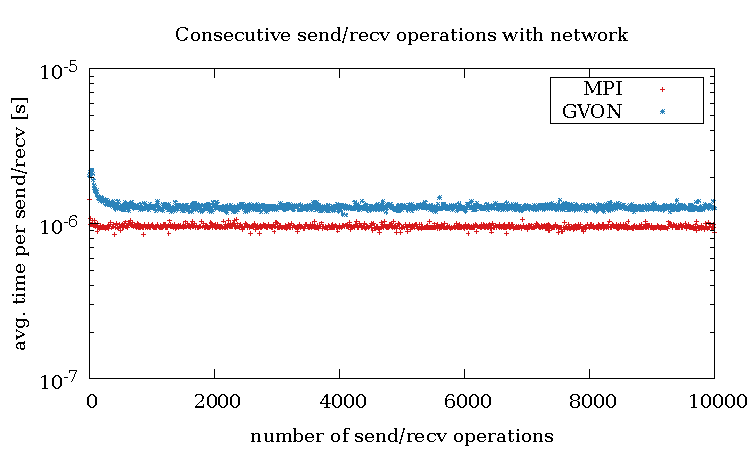
\includegraphics[width=\textwidth]{plots/50_nsend_network_gvon_laser}
    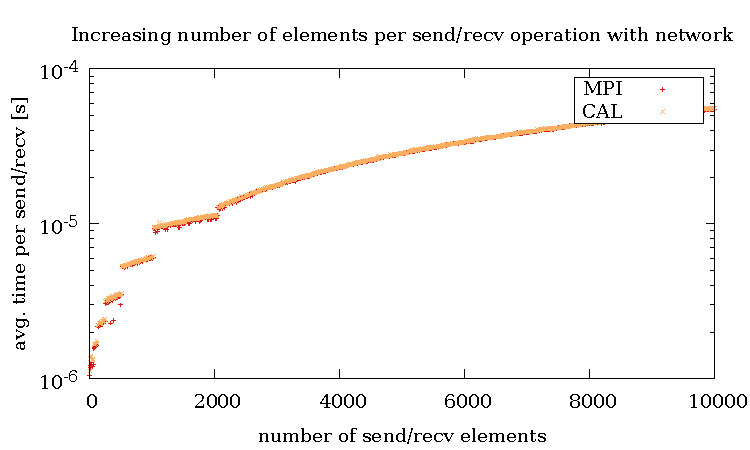
\includegraphics[width=\textwidth]{plots/50_nsize_network_cal_laser}
    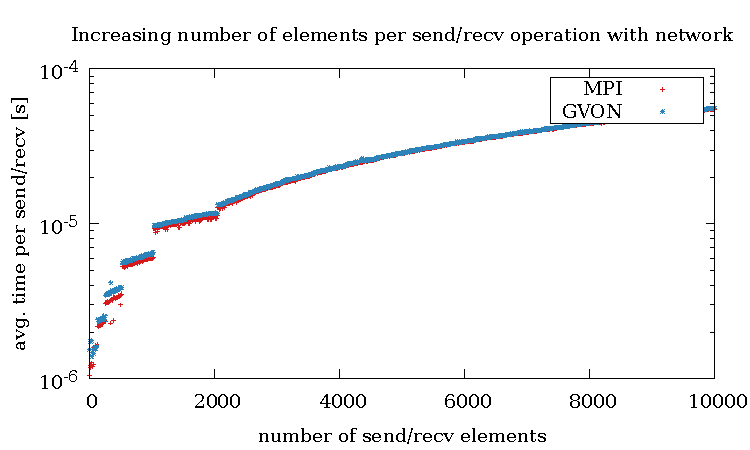
\includegraphics[width=\textwidth]{plots/50_nsize_network_gvon_laser}
    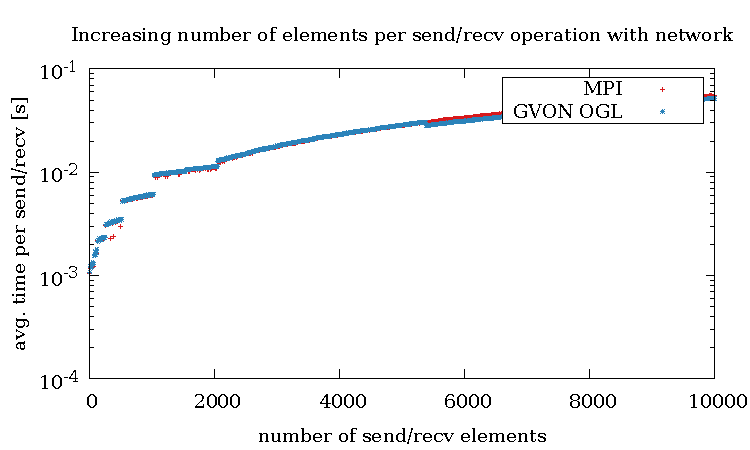
\includegraphics[width=\textwidth]{plots/50_nsize_one_lookup_network_gvon_laser}
  \end{minipage}%
  \begin{minipage}[t]{0.5\textwidth}
    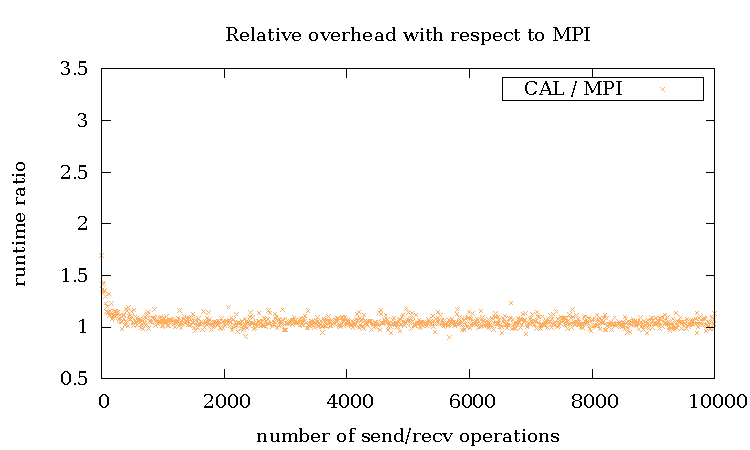
\includegraphics[width=\textwidth]{plots/50_nsend_network_overhead_cal_laser}
    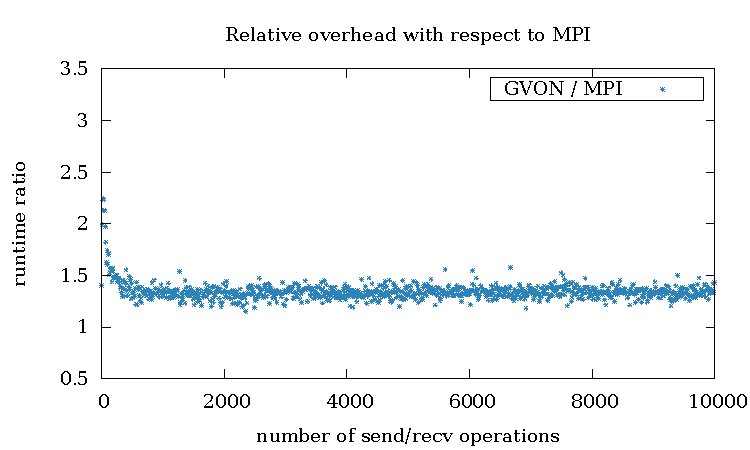
\includegraphics[width=\textwidth]{plots/50_nsend_network_overhead_gvon_laser}
    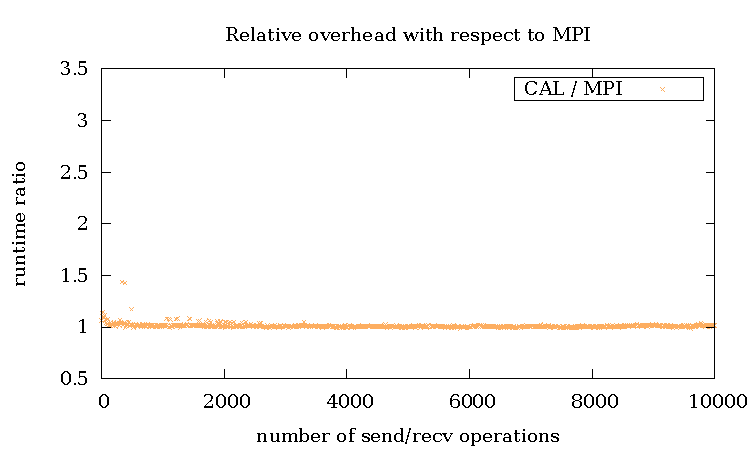
\includegraphics[width=\textwidth]{plots/50_nsize_network_overhead_cal_laser}
    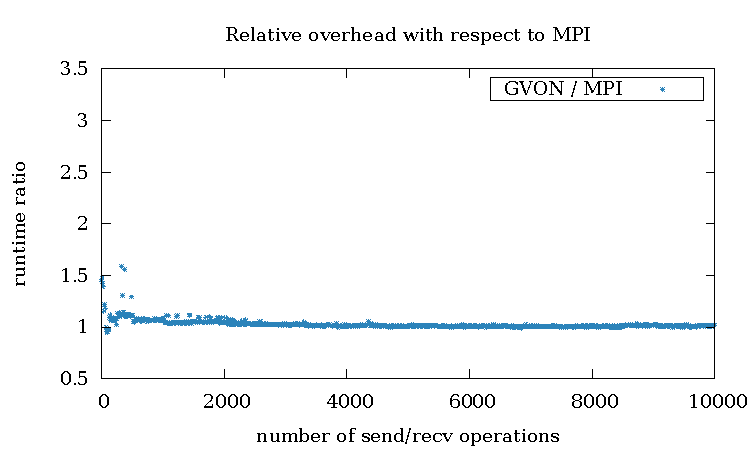
\includegraphics[width=\textwidth]{plots/50_nsize_network_overhead_gvon_laser}
        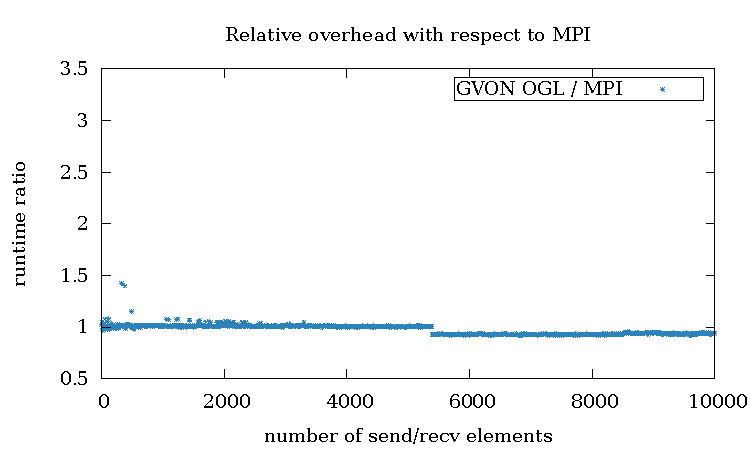
\includegraphics[width=\textwidth]{plots/50_nsize_one_lookup_network_overhead_gvon_laser}
  \end{minipage}%
  \caption{Synthetic benchmark including network latency}
  \label{fig:nsend_network}
\end{figure}

\noindent This experiment resembles more with real world simulation,
because real world simulation usually send more than a single a single
element integer per communication operation and are using a
network. Thus, the CAL and GVON overhead is in an acceptable
range.


%%%%%%%%%%%%%%%%%%%%%%%%%%%%%%%%%%%%%%%%%%%%%%%%%%%%%%%%%%%%%%%%%%%%%%%%%%%%%%%%
%                                                                              %
% SYNTHETIC COLLECTIVE BENCHMARK                                               %
%                                                                              %
%%%%%%%%%%%%%%%%%%%%%%%%%%%%%%%%%%%%%%%%%%%%%%%%%%%%%%%%%%%%%%%%%%%%%%%%%%%%%%%%
% Checked
\section{Synthetic Collective Benchmark}
This benchmark compares the run-time of MPI collectives with
equivalent collectives of the CAL and GVON.  To determine the run-time
for a single collective execution, it is averaged over executions 1000
.  Since, the overhead in respect to MPI should be determined, only
the gather and reduce collective were chosen for comparison. Other
collective operations should behave in an analog manner. The
experiments will be executed on a setup with 8 laser nodes, while the
number of peers per nodes will be increased to a maximum of 64 CPUs.
This will lead to maximum number of 512 CPUs.

\todo{increase amount of data to send}

% Checked
\subsection*{Gather Collective}
The GVON gather operation is first performed locally for all hosted
vertices of a host. Furthermore, a reordering of the gather results in
vertex index order is performed. A big relative overhead with respect
to MPI is expected.  Figure \ref{fig:gather_laser} shows the average
run-time of a gather collective for increasing number of peers with
and without network.

\begin{figure}[H]
  \begin{minipage}[t]{0.5\textwidth}
    %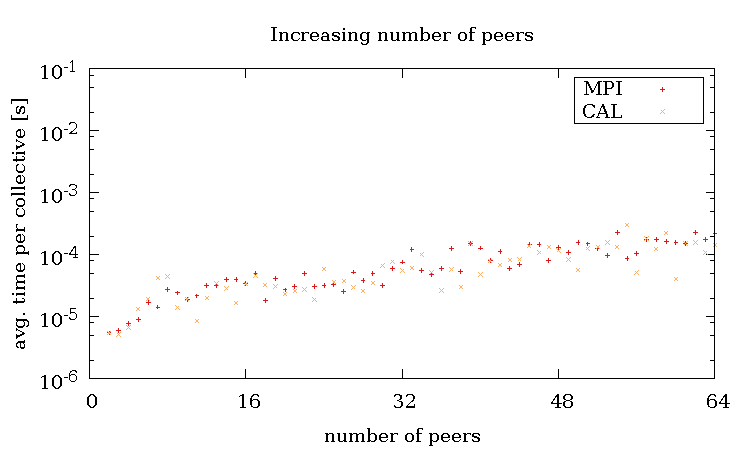
\includegraphics[width=\textwidth]{plots/50_collective_npeers_cal_laser}
    %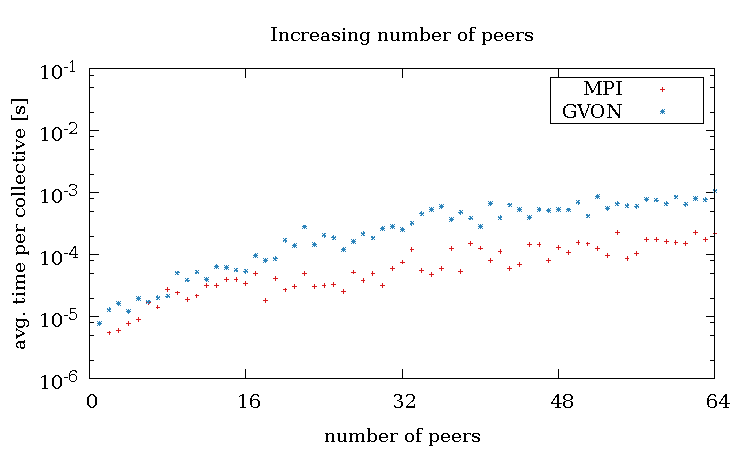
\includegraphics[width=\textwidth]{plots/50_collective_npeers_gvon_laser}
    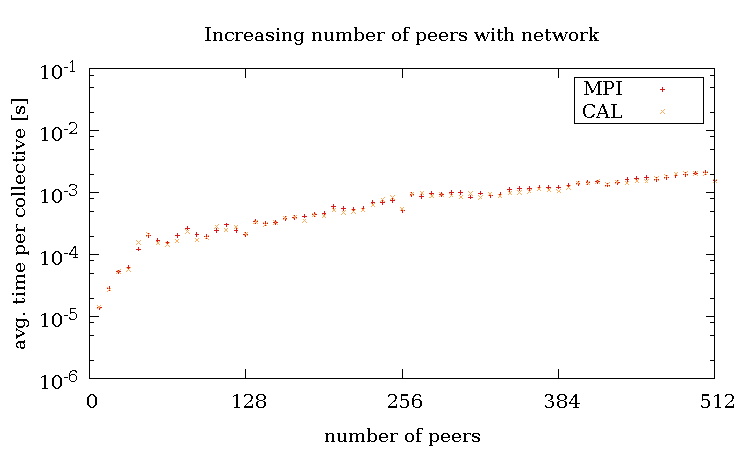
\includegraphics[width=\textwidth]{plots/50_collective_network_cal_laser}
    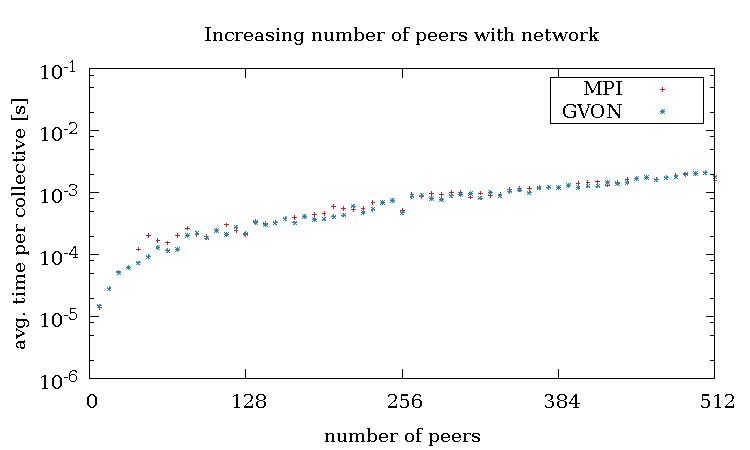
\includegraphics[width=\textwidth]{plots/50_collective_network_gvon_laser}
  \end{minipage}%
  \begin{minipage}[t]{0.5\textwidth}
    %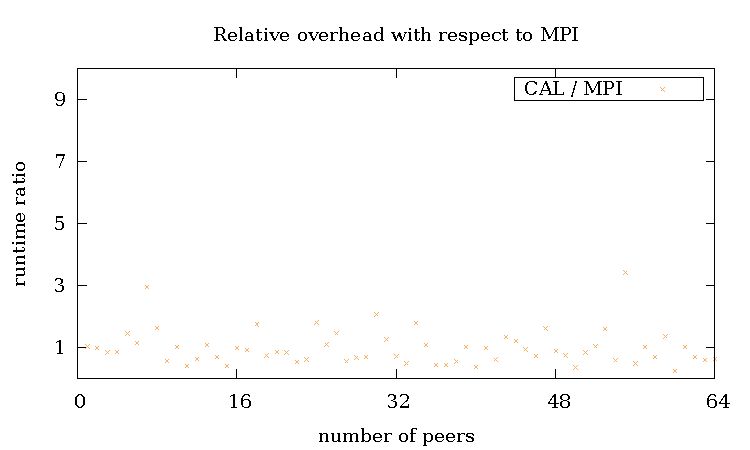
\includegraphics[width=\textwidth]{plots/50_collective_npeers_overhead_cal_laser}
    %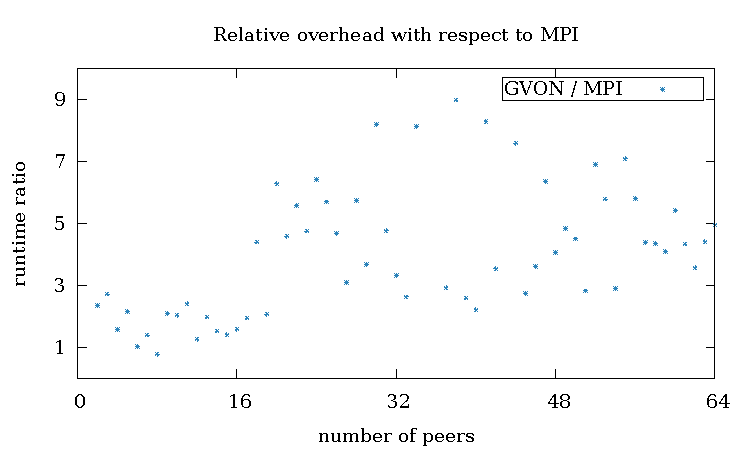
\includegraphics[width=\textwidth]{plots/50_collective_npeers_overhead_gvon_laser}
    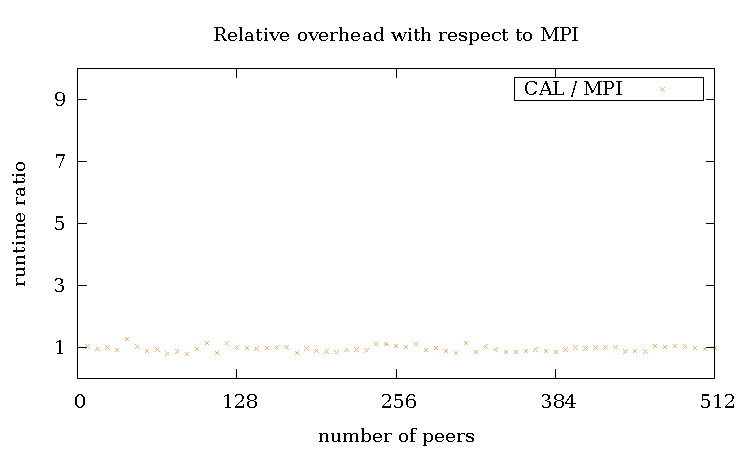
\includegraphics[width=\textwidth]{plots/50_collective_network_overhead_cal_laser}
    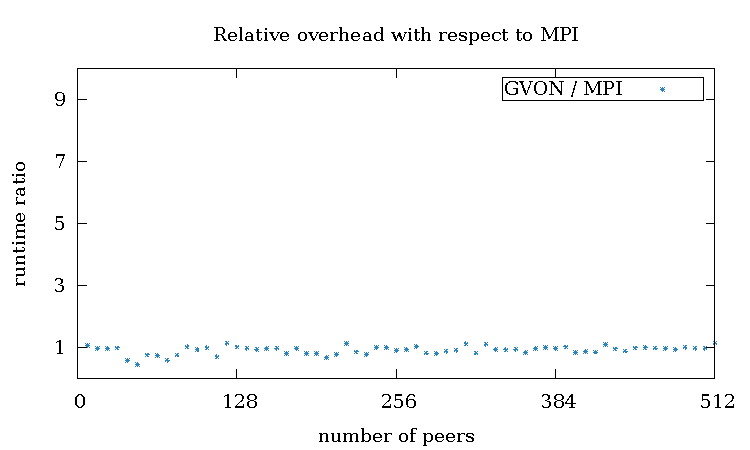
\includegraphics[width=\textwidth]{plots/50_collective_network_overhead_gvon_laser}
  \end{minipage}%
  \caption{ }
  \label{fig:gather_laser}
\end{figure}

% Checked
\subsection*{Reduce Collective}
The reduce collective of the GVON performs also a local reduce first.
Figure \ref{fig:reduce_laser} shows the average run-time of a reduce
collective for increasing number of peers with and without network.

\begin{figure}[H]
  \begin{minipage}[t]{0.5\textwidth}
    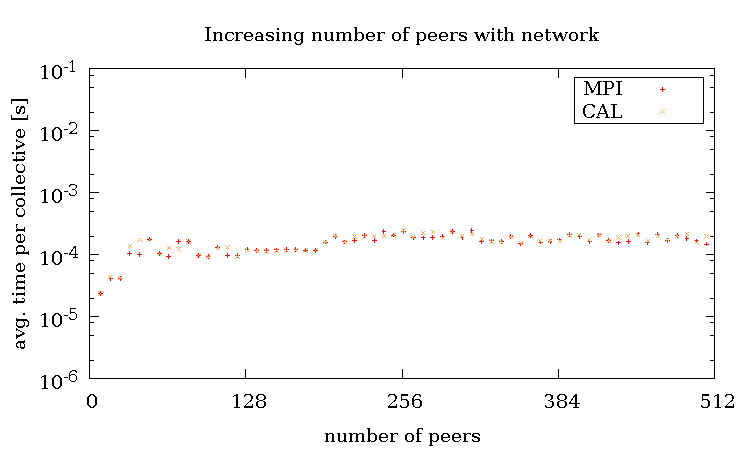
\includegraphics[width=\textwidth]{plots/50_reduce_network_cal_laser}
    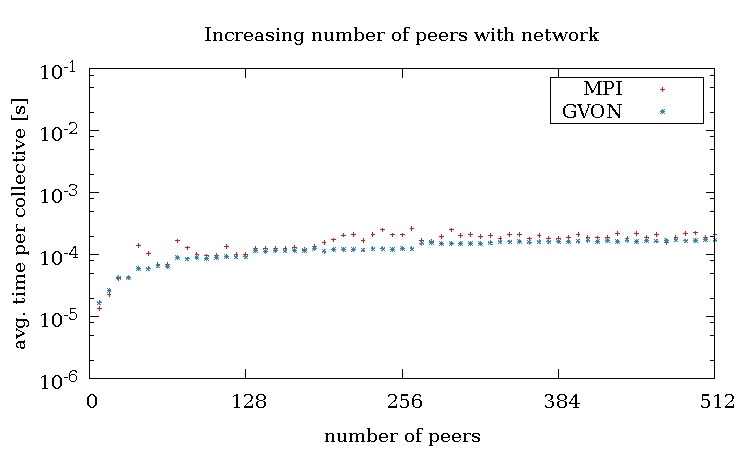
\includegraphics[width=\textwidth]{plots/50_reduce_network_gvon_laser}
  \end{minipage}%
  \begin{minipage}[t]{0.5\textwidth}
    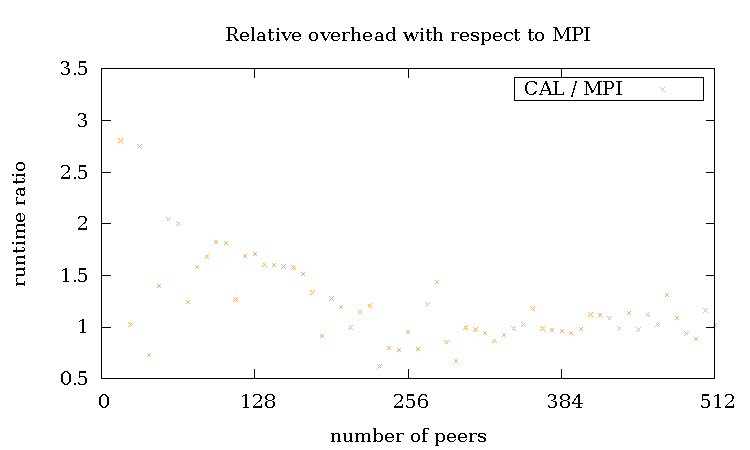
\includegraphics[width=\textwidth]{plots/50_reduce_network_overhead_cal_laser}
    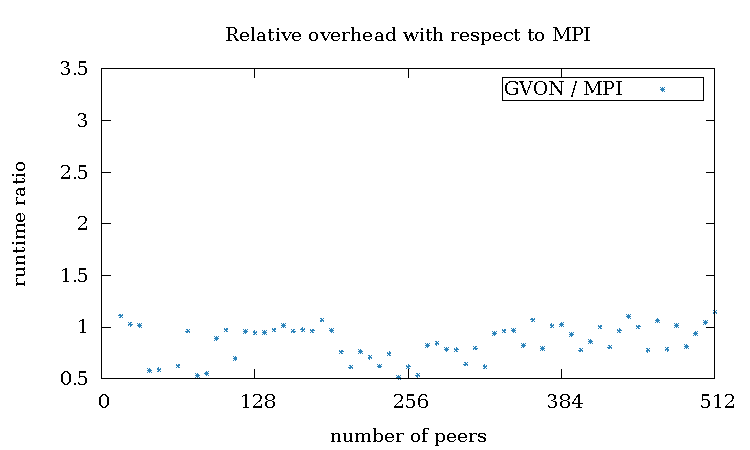
\includegraphics[width=\textwidth]{plots/50_reduce_network_overhead_gvon_laser}
  \end{minipage}%
  \caption{ }
  \label{fig:reduce_laser}
\end{figure}


%%%%%%%%%%%%%%%%%%%%%%%%%%%%%%%%%%%%%%%%%%%%%%%%%%%%%%%%%%%%%%%%%%%%%%%%%%%%%%%%
%                                                                              %
% REAL WORLD SIMULATION BENCHMARK                                              %
%                                                                              %
%%%%%%%%%%%%%%%%%%%%%%%%%%%%%%%%%%%%%%%%%%%%%%%%%%%%%%%%%%%%%%%%%%%%%%%%%%%%%%%%
% Checked
\section{Real World Simulation Benchmark}
\label{sec:eval:real}
The previous benchmarks evaluated the developed system in a very
synthetic and unreal fashion. But, real world simulation perform
usually calculations in between communication operations. Furthermore,
it is usual to overlap calculations and communication by non-blocking
operations. The Game of Life and N-body simulations were chosen as
examples for such real world simulations. The experiments compare the
implementations on top of the GVON from section \ref{sec:impl} to
equivalent MPI implementations.  Equivalent refers the same amount of
communication operations and the same functions are used to calculate
or update the simulation states. A setup with 8 laser nodes is used in
the network case. The number of peers per node is incremented for each
experiment to a maximum of 64. The peers are equally distributed to
the nodes.  Which leads to maximum number of 512 CPUs. 


%%%%%%%%%%%%%%%%%%%%%%%%%%%%%%%%%%%%%%%%%%%%%%%%%%%%%%%%%%%%%%%%%%%%%%%%%%%%%%%%
%                                                                              %
% GAME OF LIFE BENCHMARK                                                       %
%                                                                              %
%%%%%%%%%%%%%%%%%%%%%%%%%%%%%%%%%%%%%%%%%%%%%%%%%%%%%%%%%%%%%%%%%%%%%%%%%%%%%%%%
% Checked
\subsection{Game of Life Benchmark}
This experiment compares the GVON implementation of Game of Life from
section \ref{sec:gol} with an equivalent MPI implementation. The GoL
domain is a rectangular field and the state of every cell is
calculated exclusively by one peer. The average run-time for a
time-step with increasing number of cells is measured. The run-time is
measured with and without network influence.  Figure
\ref{fig:gol_laser} shows the average run-time of a time-step with and
without network.

\begin{figure}[H]
    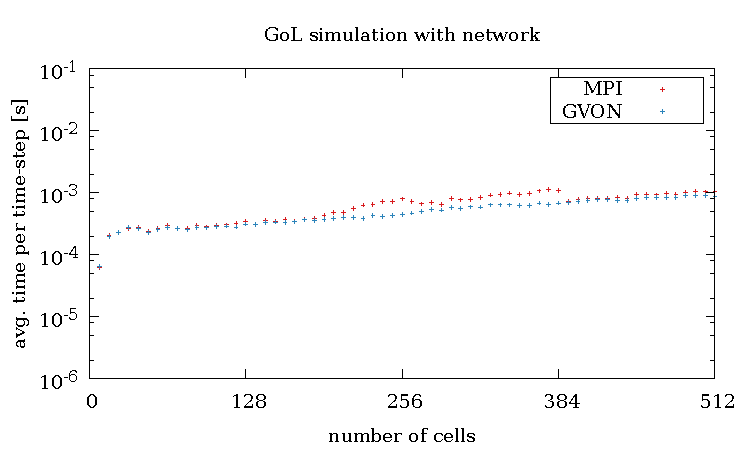
\includegraphics[width=\textwidth]{plots/50_gol_network_laser}
  \label{fig:gol_laser}
  \caption{Average run-time of GoL simulation with increasing number
    of cells. The simulation is executed with network.}
\end{figure}

The GVON implementation shows no overhead in comparison to the MPI
implementation.


%%%%%%%%%%%%%%%%%%%%%%%%%%%%%%%%%%%%%%%%%%%%%%%%%%%%%%%%%%%%%%%%%%%%%%%%%%%%%%%%
%                                                                              %
% N BODY BENCHMARK                                                             %
%                                                                              %
%%%%%%%%%%%%%%%%%%%%%%%%%%%%%%%%%%%%%%%%%%%%%%%%%%%%%%%%%%%%%%%%%%%%%%%%%%%%%%%%
% Checked
\subsection{N-Body Benchmark}
This benchmark simulates the implemented N-body simulation for 1000
time-steps with increasing number of bodies. It is compared a
simulation implemented with MPI to one implemented with the GVON.
Thereby, each body is managed by an own peer. Thus, the number of
peers increases with the number of bodies. The experiment is performed
with and without network. Figure \ref{fig:nbody_laser} shows the
averaged run-time of a time-step with increasing number of bodies with
and without network.

\begin{figure}[H]
  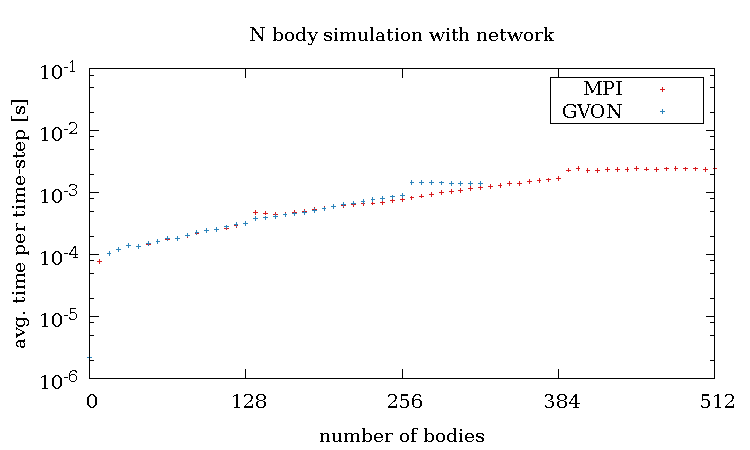
\includegraphics[width=\textwidth]{plots/50_nbody_network_laser}
  \label{fig:nbody_laser}
  \caption{Average run-time of N-body simulation with increasing
    number of bodies. The simulation is executed with network.}
\end{figure}

Analog to the GoL simulation, this experiment also shows no overhead
in comparison to the MPI implementation.

%%%%%%%%%%%%%%%%%%%%%%%%%%%%%%%%%%%%%%%%%%%%%%%%%%%%%%%%%%%%%%%%%%%%%%%%%%%%%%%%
%                                                                              %
% FLEXIBILITY BENCHMARK                                                        %
%                                                                              %
%%%%%%%%%%%%%%%%%%%%%%%%%%%%%%%%%%%%%%%%%%%%%%%%%%%%%%%%%%%%%%%%%%%%%%%%%%%%%%%%
\section{Flexibility Benchmark}
\todo{Write flexibility benchmark}
\begin{itemize}
\item GVON allows mapping of vertices to peers at run-time
\item Remapping of vertices possible
\item Furthermore, mapping of multiple vertices onto a single peer
\end{itemize}


%%%%%%%%%%%%%%%%%%%%%%%%%%%%%%%%%%%%%%%%%%%%%%%%%%%%%%%%%%%%%%%%%%%%%%%%%%%%%%%%
%                                                                              %
% CONCLUSION                                                                   %
%                                                                              %
%%%%%%%%%%%%%%%%%%%%%%%%%%%%%%%%%%%%%%%%%%%%%%%%%%%%%%%%%%%%%%%%%%%%%%%%%%%%%%%%

\cleardoublepage

%%% Local Variables:
%%% TeX-master: "diplom"
%%% End:
